\documentclass[10pt]{article}

\def\Type{LessonCaelan}
\def\TypeNum{Lesson 5}
\def\TypeTitle{Derivatives \& Rates of Change }
\def\Semester{Fall 2021} %Not Used 
\def\Course{MATH 1190 \& 1210}
\def\Targets{ {\bf\color{ForestGreen}D1} }
\def\desmosClassCode{{\bf ZAJ$3$AZ}}
\usepackage{preambleDJ}




%%%%%%%%%%%% BEGIN DOCUMENT %%%%%%%%%%%%%%%
%%%%%%%%%%%% BEGIN DOCUMENT %%%%%%%%%%%%%%%
%%%%%%%%%%%% BEGIN DOCUMENT %%%%%%%%%%%%%%%
%%%%%%%%%%%% BEGIN DOCUMENT %%%%%%%%%%%%%%%
%%%%%%%%%%%% BEGIN DOCUMENT %%%%%%%%%%%%%%%

\begin{document}

\thispagestyle{empty}

\Heading{MATH 1190 \& 1210 Survey of Calculus I}{\begin{minipage}{0.25\textwidth}\begin{center} Week 4 Workshop \end{center}\end{minipage}}

\vspace{0.1in}

\Name{}
\vspace{0.3cm}

In this worksheet, you will estimate the derivative of functions at various points, then use those estimates to guess at the general formula of the ``derivative machine" function that generates them.

\begin{enumerate}
    \item Consider the function $f(x) = x^2$.
    \begin{enumerate}
        \item We want to compute the derivative \[f'(a) = \lim_{h\to 0}\frac{f(a+h) - f(a)}{h}\]
        for various values of $a$. Feel free to use any techniques we've seen to compute these limits. Some things you can try are:
        \begin{itemize}
            \item compute the quantity for very small values of $h$,
            \item use algebraic manipulations to simplify, or
            \item find a line with slope equal to the result of the limit and estimate that.
        \end{itemize}
        Record your answers here, and show your work on a separate page.
        \[
            \arraycolsep=20pt
            \begin{array}{c|ccccc}
                a & -2 & -1 & 0 & 1 & 2 \\ \hline
                f'(a) & 
            \end{array}
        \]
\vspace{0.5cm}
        \item Now, plot the values you found as points $\big(a,f'(a)\big)$ below.
        \begin{center}
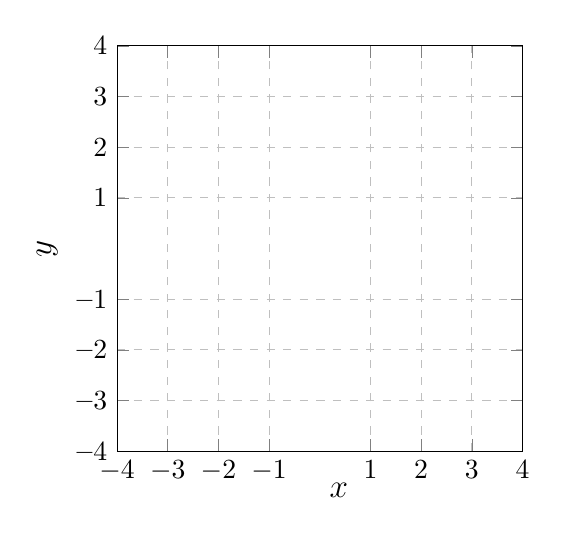
\begin{tikzpicture}[]
      \begin{axis}[
    %    axis y line = left,
    %    axis x line = bottom,
        xlabel = {\large$x$},
                        xlabel style={anchor=west},
        ylabel = {\large$y$},
                        ylabel style={anchor=south},
        xtick       = {-4,-3,-2,-1,1,2,3,4},
        xticklabels = {$-4$,$-3$,$-2$,$-1$,$1$,$2$,$3$,$4$},
        ytick       = {-4,-3,-2,-1,1,2,3,4},
        yticklabels = {\textbf{--}$4$,\textbf{--}$3$,\textbf{--}$2$,\textbf{--}$1$,$1$,$2$,$3$,$4$},
        samples     = 160,
        domain      = 0:3,
        restrict y to domain=-10:100,
        xmin = -4, xmax = 4,
        ymin = -4, ymax = 4,
        width=2.65in,height=2.65in,
        grid=both, grid style=dashed
      ]
    \end{axis}
\end{tikzpicture}
\end{center}
\item Based on this data, what equation do you think describes the function which takes a number $a$ and outputs $f'(a)$?
\vspace{2cm}

\end{enumerate}
\item If you have time: try this process for another function. Pick your favorite below:
\begin{enumerate}
    \item (Easier) $f(x)=mx+b$ for any $m$ and $b$
    \item (Medium) $f(x) = x^3$
    \item (Harder) $f(x) = 2^x$ or $f(x) = \ln(x)$
\end{enumerate}
\end{enumerate}
\end{document}
